\begin{boxD}
پیاده‌سازی یک روش نهان‌کاوی به عنوان آشکارسازی بر نهان‌نگاری به روش
\grayBox{\lr{LSB}}
.

یعنی فرض‌کنید که ما با روش
\grayBox{\lr{LSB}}
عملیات نهان‌نگاری را انجام دادیم شما باید یک روش نهان‌کاوی به منظور تشخیص آن پیاده‌سازی کنید.
\end{boxD}

\begin{boxA}
طبق الگوریتم این روش نهان‌نگاری ابتدا تک تک بیت های پیام رمز
\grayBox{\lr{CipherText}}
را در کم ارزش‌ترین بیت های پیکسل های موجود در عکس قرار‌می‌دهیم.

ابتدا باید پیام مدنظر خود را که در زیر آمده‌است را باید در تصویر پنهان کنیم.
در کد پایتون زیر این عملیات را با استفاده از عملگرهای بیتی انجام داده ایم.

\grayBox{\lr{Shahid Ghasem Soleimani}}
\end{boxA}

\begin{boxE}
    \lr{\lstinputlisting[language=Python]{security_images/hide.py}}
\end{boxE}

\begin{boxA}
     همانطور که در کد بالا ، که برای پنهان‌سازی پیام می‌باشد ، مشاهده‌می‌کنید :
     برای جاگذاری بیت‌های پیام به جای کم‌ارزش‌ترین بیت هر پیکسل ، 
     ابتدا می‌بایستی بیت‌آخر هر پیکسل را نابود کنیم.

     یا به عبارت بهتر ، بیت آخر هر پیکسل را صفر قرار دهیم.
     این کار با یک عملیات 
    \grayBox{\lr{AND}}
     منطقی صورت می‌پذیرد.
     (\grayBox{\lr{pixel[n] and ~1}})

     \newline
    
     سپس با عملیات 
     \grayBox{\lr{OR}}
     منطقی ، بیت پیام را در جایگاه مدنظر قرارخواهیم داد.
     % \newline
     % (\grayBox{\lr{(pixel[n] and ~1) or int(b_message[index])}})

     و همینطور بالعکس ، برای آشکارسازی این پیام نهفته‌شده می‌بایستی که ابتدا تمام بیت‌های کم‌ارزش را استخراج کنیم.
     سپس تا زمانی که به رشته
     \grayBox{\lr{Tamam}}
     برخورد نکرده‌ایم ، این مجموعه رشته باینری را به کداسکی متناظر تبدیل میکنیم.

     نکته مهم در اینجا این است که طبیعتا تعداد پیکسل‌های تصویر ما بسیار بیشتر از تعداد بیت‌های پیام ما خواهد بود.
     
     برای این منظور باید به گیرنده،  با یک پیام مشخص ،انتهای پیام خود را 
    نشان‌دهیم.

    این پیام در این تمرین
    \grayBox{\lr{Tamam}}
    خواهد بود.

\end{boxA}

\begin{boxE}
    \lr{\lstinputlisting[language=Python]{security_images/unhide.py}}
\end{boxE}

\begin{figure}[h]
    \centering
    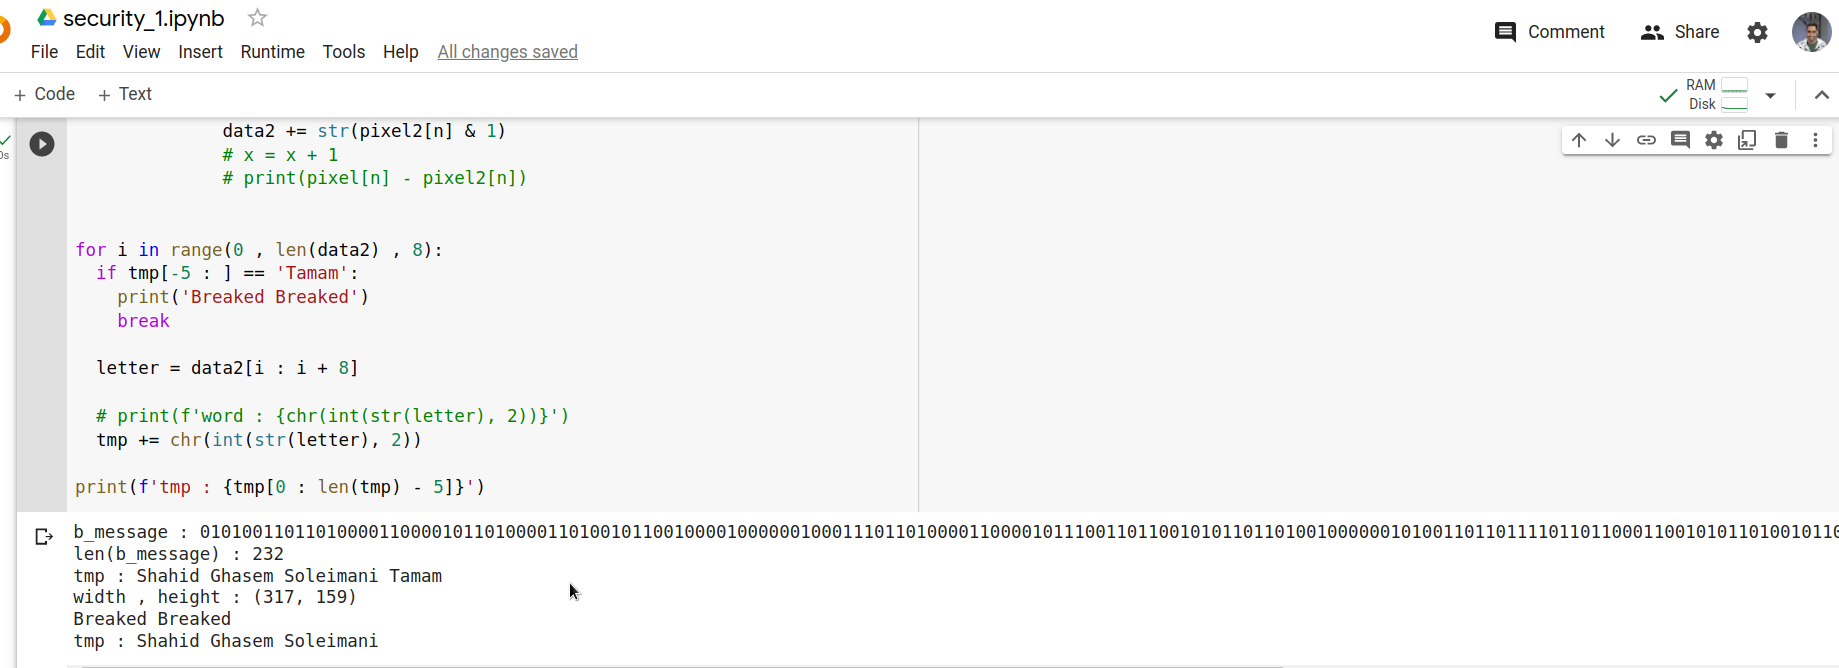
\includegraphics[width=0.95\textwidth ]{security_images/hideandunhide.png}
    % [width=0.5\textwidth , height = 0.5\textwidth]
    \caption{
    پنهان‌کردن و آشکارکردن پیام
    \grayBox{\lr{Shahid Ghasem Soleimani}}
    }
    \label{fig:my_label}
\end{figure}

\begin{figure}[h]
    \centering
    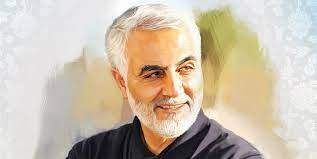
\includegraphics[width=0.85\textwidth]{security_images/shahid_soleimani.jpeg}
    % [width=0.85\textwidth]
    \caption{تصویری که بر روی آن 
    \grayBox{\lr{steganography}}
    را انجام داده‌ایم
    }
    \label{fig:my_label}
\end{figure}